	\documentclass[twoside]{article}
\usepackage{../../estilo-ejercicios}
\setcounter{section}{0}
\newtheorem{defin}{Definition}[section]
\newtheorem{lem}[defin]{Lemma}
\newtheorem{propo}[defin]{Proposition}
\newtheorem{thm}[defin]{Theorem}
\newtheorem{eje}[defin]{Example}
\newtheorem{obs}[defin]{Observación}
\renewcommand{\baselinestretch}{1,3}
%--------------------------------------------------------
\begin{document}

\title{Characterization of Extremal Antipodal Polygons}
\author{Javier Aguilar Martín}
\maketitle

%\varprojlim
%\varinjlim
\section{Introduction}

For a point $p=(x_1,x_2)\in\R^2$, let $p'=(-x_1,-x_2)$ be the antipodal point of $p$.

\begin{defin}
A set of $2n$ ($n\geq 3$) points on the unit circle centered at the origin is called an \emph{antipodal point set} if for every point $p\in S$, also $p'\in S$. Let $S=\{p_1,p_1'\dots,p_n,p_n'\}$ such set. An \emph{antipodal polygon} on $S$ is a convex polygon  having as vertices one point for each pair $(p_i,p_i')$. A \emph{thin} antipodal polygon $P$ is an antipodal polygon whose verticies are consectuvie points on the circle. For $n$ odd, a \emph{thick} antipodal polygon $P$ is an antipodal polygon such that there is a point of $S$ between every two vertices of $P$. For $n$ even there is exactly one pair of vertices of $P$ which are consecutive on the circle. 
\end{defin}

\begin{figure}[h!]
\centering
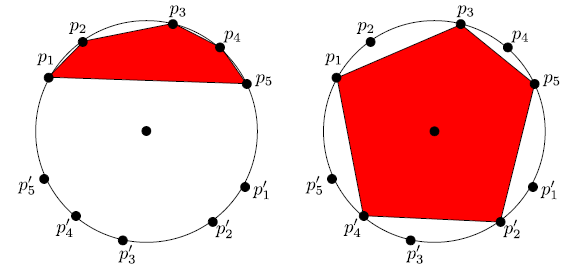
\includegraphics[scale=0.7]{fig1}
\caption{A thin (left) and a thick (right) antipodal polygon.}
\end{figure}
 
 
 Note that an antipodal polygon $P$ can be neither thick or thin, but it cannot be both at the same time. Moreover, a thin antipodal polygon does not contain the origin and a non-thin polygon always contains it (not choosing one point of $S$ implies choosing its antipodal). 
 
We will consider the following questions:
\begin{itemize}
\item Does a thick antipodal polygon always have larger area than a thin antipodal polygon?
\item How efficiently can one compute an antipodal polygon with minimal (maximal)
area?
\item What can be said about antipodal polygons in higher dimensions?
%•
\end{itemize}

\subsection{Related Work}

\subsection{Results}\label{claim}
We will prove the following general result:

\emph{Claim} Given an antipodal point set $S ⊂ \R^2$, every thin antipodal polygon on $S$ has
less area than any non-thin antipodal polygon on $S$.

In addition we show that the 2-dimensional case is special in the sense that the
above result can not be generalized to higher dimensions.

The analogue result holds for thick antipodal polygons when $n$ is odd but for $n$ even we provide an example of
an antipodal non-thick polygon having larger area than a thick antipodal polygon. However, we are able to prove the following result:

\emph{Claim} Given an antipodal point set $S ⊂ \R^2$, for every non-thick antipodal polygon
on $S$ there exists a thick antipodal polygon on $S$ with larger area.

Note that above claims imply that an antipodal polygon with minimum (resp. maximum)
area is thin (resp. thick). As a consequence, we will show that the extremal
problems for antipodal polygons can be solved in linear time.

\section{Thin Antipodal Polygons}
Assume that the clockwise circular order of $S$ around the origin is $p_1, p_2, \dots , p_n,
p'_1, p'_2,\dots , p'_n$. For every point $q$ in $S$, let $P_q$ be the thin antipodal polygon that
contains as vertices $q$ and the next $n −1$ clockwise consecutive points of $S$. Note that
all thin antipodal polygons are of this form and that $P_q$ and $P_{q'}$ differ only by a rotation around the origin. 

The next lemma characterizes triangles that contain a given point of S and maximize
the area.

\begin{lem}
For a point $p ∈ S$ let $l$ be the line containing $p$ and $p'$. Let $τ$ be the triangle
determined by $p$, and its two neighbors in $S$. Among all triangles that have as vertices
$p$ and one point of $S$ in each of the two half-planes defined by $l$, $τ$ has strictly the
smallest area.
\end{lem}

SI VEO QUE DA TIEMPO PONER LAS PRUEBAS DE LOS LEMAS QUE SON CORTAS. O ALTERNATIVAMENTE NO PONER LAS PRUEBAS PERO EXPLICAR EL PÁRRAFO QUE VIENE DESPUÉS ANTES DEL TEOREMA

We split the proof of the first claim of \ref{claim} into the three cases $n = 3$, $n = 4$, and $n ≥ 5$.

\begin{lem}
For $n = 3$, every thin antipodal polygon on $S$ has area strictly less than
that of any non-thin antipodal polygon on $S$.
\end{lem}

\begin{lem}
For $n = 4$, every thin antipodal polygon on $S$ has area strictly less than
that of any non-thin antipodal polygon on $S$.
\end{lem}

\begin{thm}
Every thin antipodal polygon on $S$ has less area than any non-thin antipodal
polygon on $S$.
\end{thm}


\section{Thick Antipodal Polygons}
ULISES

\section{Higher Dimensions: Antipodal Polytopes}
ULISES


 \section{Open Problems}
 NO LO ENTIENDO, PREGUNTARLE AL PROFESOR
\end{document}
